\documentclass[10pt]{article}

\usepackage[utf8]{inputenc}
\usepackage[french]{babel}
\usepackage{amsmath}
\usepackage{amsfonts}
\usepackage{amssymb}
\usepackage{graphicx}
\usepackage{parskip}


\begin{document}

\title{IFT2425 - TP3 - Rapport}
\date{Mars 2011}
\author{Vincent Foley-Bourgon (FOLV08078309) \and
  Eric Thivierge (THIE09016601)}

\maketitle

\section{Interpolation}

\subsection{Description du problème et méthodes utilisées}

Étant donné la fonction $\sin(x)$ sur l'intervalle $[0, 3\pi]$, on doit
trouver des polynômes de collocation d'ordre 1 à 5 qui approximent
cette fonction.  Comme on peut choisir des points équidistants, nous
avons choisi de trouver les polynômes avec la méthode de
Newton-Grégory.

La fonction \emph{InterpolationPolynomialNew} s'occupe de créer ce
polynôme: elle prend en paramètres une fonction $f$ qui sert à créer
un tableau de points, un entier positif \emph{degree} qui donne
l'ordre désiré du polynôme et deux valeurs flottantes, \emph{start} et
\emph{end}, qui définissent l'intervalle désiré.

Comme les polynômes de collocation de la méthode Newton-Grégory ont la
forme suivante:

\[
P(x) = c_0 + c_1(x-x_0) + \frac{c_2(x-x_0)(x-x_1)}{2!} + ...
\]

Et que de faire le développement d'un polynôme se fait en temps
$O(n^2)$, nous avons choisi de ne pas regrouper les termes et de
plutôt écrire une fonction spéciale
\emph{InterpolationPolynomialPrint} pour faire l'affichage des
polynômes de collocation.

\subsection{Graphes de l'erreur des polynômes d'interpolation}

Les graphiques suivants montrent l'erreur absolue faite entre
l'approximation par polynôme et la fonction $\sin$.  On remarque au
fur et à mesure que l'on ajoute des termes au polynôme, l'erreur
absolue diminue.

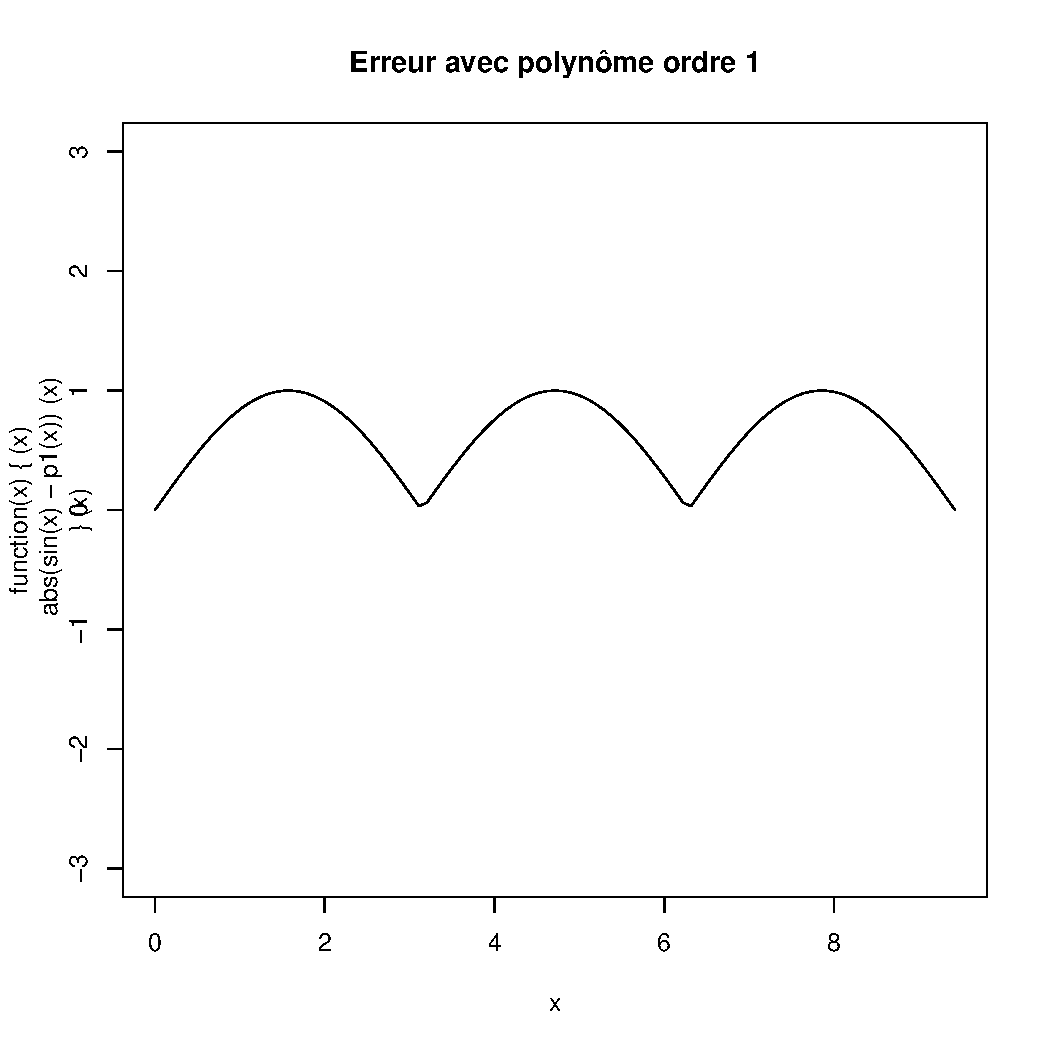
\includegraphics[scale=0.4]{data/p1}
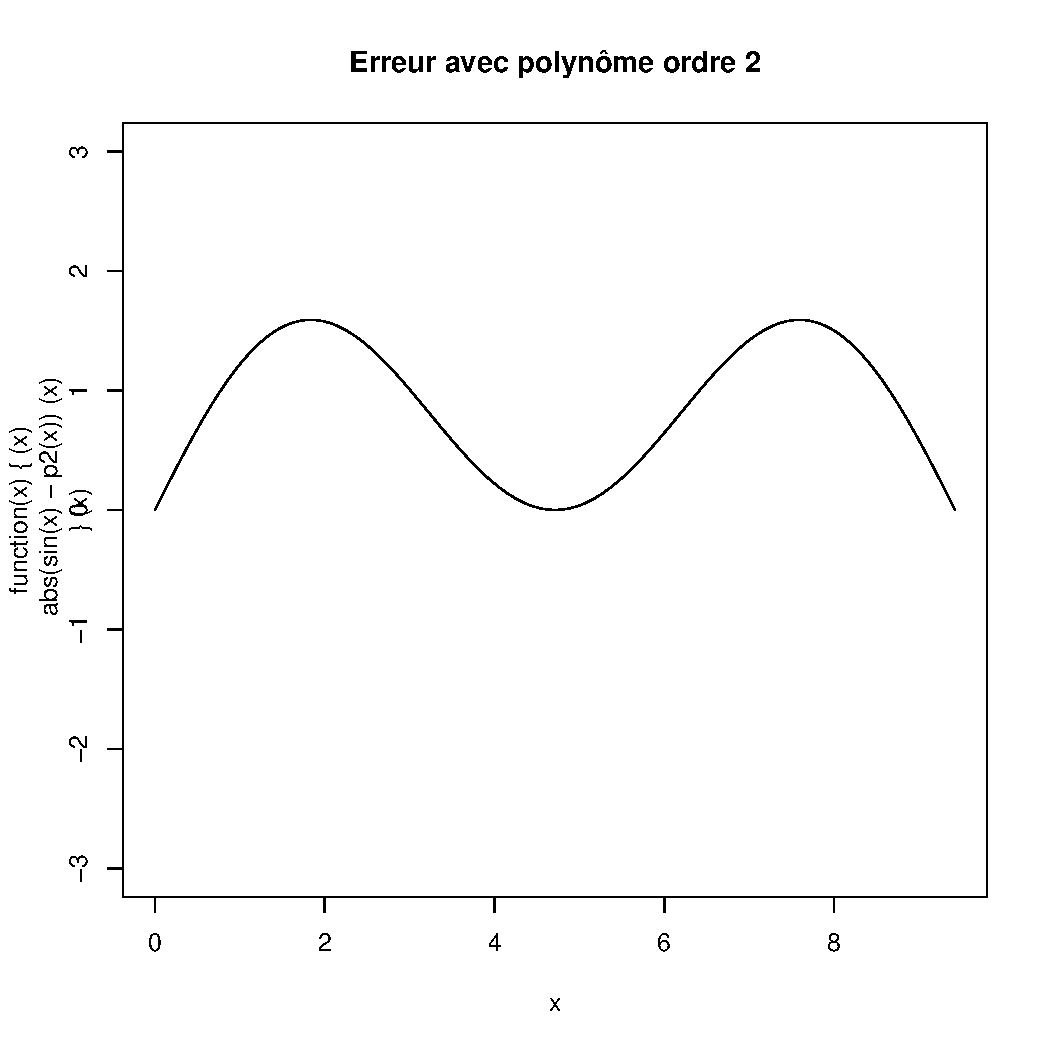
\includegraphics[scale=0.4]{data/p2}
\includegraphics[scale=0.4]{data/p3}
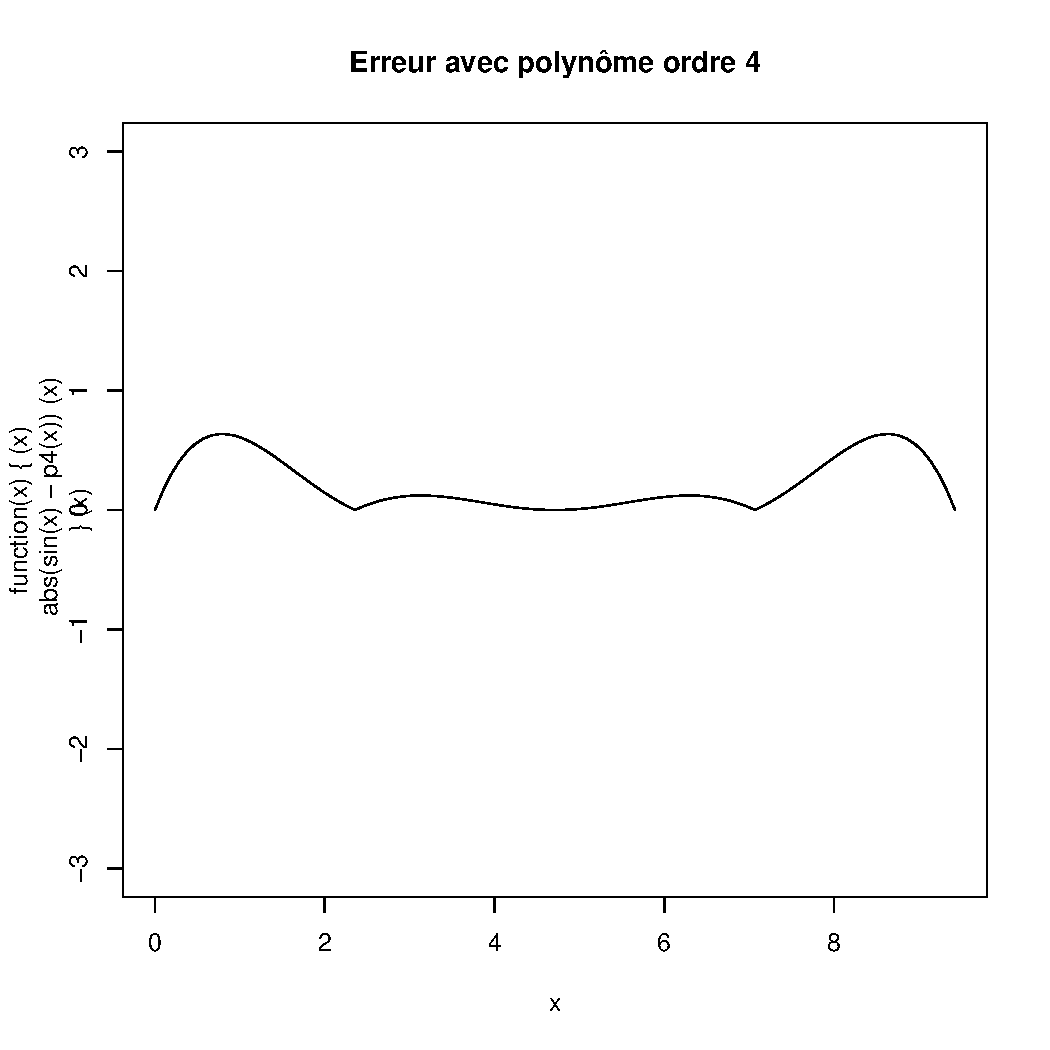
\includegraphics[scale=0.4]{data/p4}
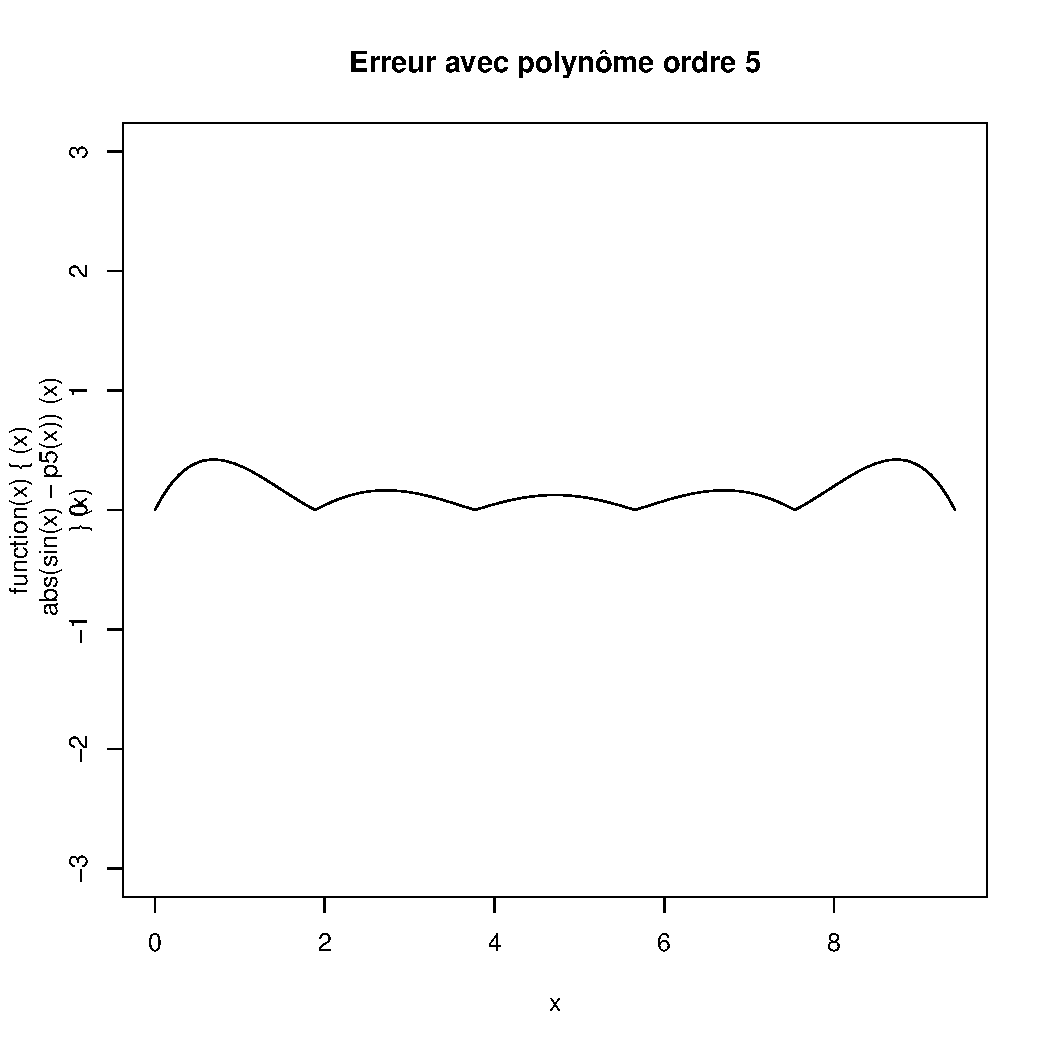
\includegraphics[scale=0.4]{data/p5}


\section{Intégration numérique}

\subsection{Description du problème et méthodes utilisées}

Le problème demande de faire la résolution numérique de l'intégrale
suivante:

\[
\int_0^1 \frac{1}{x^2 + x + 1}dx
\]

en utilisant les méthodes suivantes:

\begin{itemize}
\item Méthode des trapèzes
\item Méthode de Simpson 1/3
\item Méthode de Simpson 3/8
\end{itemize}

L'utilisateur spécifie le nombre d'intervalles à utiliser; on utilise
ce nombre directement dans la méthode des trapèzes, et pour les
méthodes de Simpson, on procède comme suit:

\begin{itemize}
\item Si le nombre d'intervalles est pair, on utilise uniquement la
  méthode de Simpson 1/3;
\item Si le nombre d'intervalles est impair, on utilise la méthode de
  Simpson 3/8 sur les 3 derniers intervalles et Simpson 1/3 sur les autres.
\end{itemize}

\subsection{Réponse aux questions}

La solution analytique de l'intégrale est $\pi/3\sqrt{3} = 0.6046$.  En
augmentant progressivement le nombre d'intervalles, les deux méthodes
(trapèzes et Simpson) convergent vers cette solution.  En examinant le
graphique ci-dessous, on peut remarquer que la méthode de Simpson
converge plus rapidement que la méthode des trapèzes.

\includegraphics[scale=0.8]{delta.pdf}


\end{document}
